\documentclass[11pt,a4paper]{report}
\usepackage[utf8]{inputenc}
\usepackage[french]{babel}
\usepackage[T1]{fontenc}
\usepackage{amsmath}
\usepackage{amsfonts}
\usepackage{amssymb}
\usepackage{xcolor}
\usepackage{gensymb}

\usepackage{geometry}
\geometry{hmargin=2.5cm,vmargin=1.5cm}
\usepackage{wasysym}
\usepackage{graphicx}

\author{Mathieu Sarrat}
\title{LC4 - Synthèses inorganiques}

\makeatletter
\renewcommand{\thesection}{\@arabic\c@section}
\makeatother


\begin{document}
\maketitle

\section*{Niveau, Pré-requis et objectifs}
\begin{itemize}
	\item \textbf{Niveau :} Terminale STL, option SPCL \\
	
	\item \textbf{Pré-requis :}
	\begin{itemize}
		\item Représentation de Lewis
		\item Acides et bases
		\item Titrage direct par colorimétrie		
		\item Tableau d'avancement\\
	\end{itemize}
	
	\item \textbf{Objectifs :}
	\begin{itemize}
		\item Notions sur les complexes : centre, ligand, liaison de coordination, 
			constante de formation;
		\item Synthèse et analyse d'un complexe;
		\item Étude documentaire d'une synthèse industrielle.\\
	\end{itemize}
		
	\item \textbf{Matériel :}
	\begin{itemize}
		\item balance de précision
		\item dispositif de filtration sous vide
		\item plaque chauffante (si possible avec contrôle de température)
		\item thermomètre
		\item \textbf{deux} burettes de 30 mL\\
	\end{itemize}
		
	\item \textbf{Recommandations :}
	\begin{itemize}
		\item 
	\end{itemize}
\end{itemize}

\newpage
\section*{Introduction}



%\begin{figure}[h!]
%	\begin{center}
%		\begin{tabular}{cc}
%  		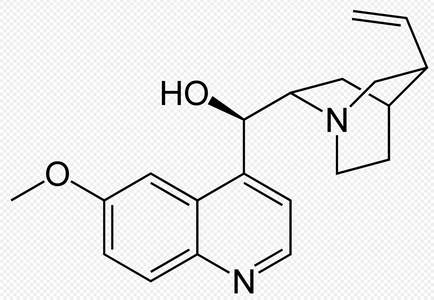
\includegraphics[scale = 0.7]{quinine.png} &
%   		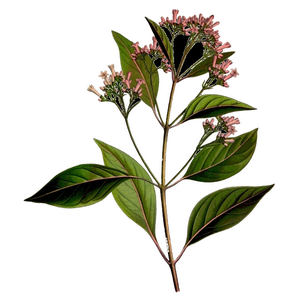
\includegraphics[scale = 0.7]{quinquina.png}\\
%   		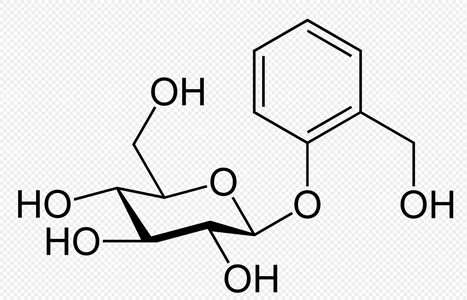
\includegraphics[scale = 0.7]{salicyline.png} &
%   		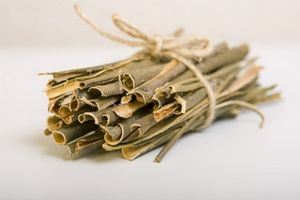
\includegraphics[scale = 0.7]{saule.png}\\
%	\end{tabular}
%	\caption{En haut, quinine et quinquina. En bas, salicyline et écorce de saule.}
%	\end{center}
%\end{figure}

\newpage
\section{Les complexes}\label{sec:1}

\subsection{Définition et structure d'un complexe}

\textbf{Définition :} un complexe est un édifice polyatomique constitué d'un \textbf{atome ou d'un ion central} auquel sont liés des molécules ou des ions appelés \textbf{ligands}. On les appelle aussi composés de coordination.

\textbf{L'atome ou ion central} doit pouvoir \textbf{accepter des doublets électroniques}. C'est le plus souvent un atome ou un cation métallique :
\begin{equation}
	\text{Cu}^{2+},\;\text{Fe}^{2+},\;\text{Ni}^{2+},\;\text{Co}^{2+},\;\text{Fe}^{3+},\;
	\text{Ni},\;\text{Co},\;\text{Fe}.
\end{equation}

\textbf{Les ligands} sont des molécules ou des ions \textbf{possédant au moins un doublet non liant}. Ils sont \textbf{monodentates} s'ils se fixent à l'atome central par un seul doublet \textcolor{red}{(dessiner les formules de Lewis avec les doublets non liants au tableau)},
\begin{equation}
	\text{H}_2\text{O},\;\text{NH}_3,\;\text{Cl}^-,\;\text{CO},\;\text{CN}^-,\;
	\text{I}^-,\;\text{HO}^-
\end{equation}
et \textbf{polydentates} s'ils se fixent à l'atome central via plusieurs doublets :
\begin{itemize}
	\item 1,2-diaminoéthane (ou éthylènediamine) est un ligand bidentate;
	\item l'ion $\text{Y}^{4-}$, base conjuguée de l'EDTA (éthylènediaminetétraacétique), est un 				ligand hexadentate.
\end{itemize}

\begin{figure}[h!]
	\begin{center}
		\begin{tabular}{cc}
  		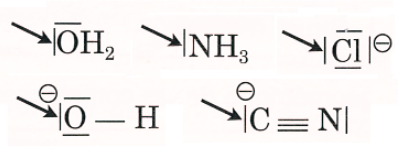
\includegraphics[scale = 0.4]{monodentate.png} &
   		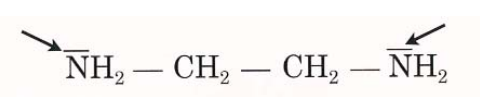
\includegraphics[scale = 0.4]{ethylenediamine.png}\\
   		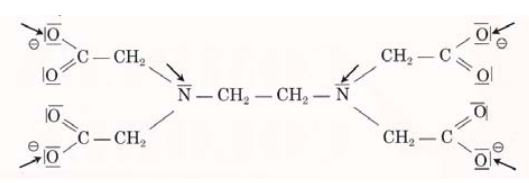
\includegraphics[scale = 0.5]{sel_edta.png} &
   		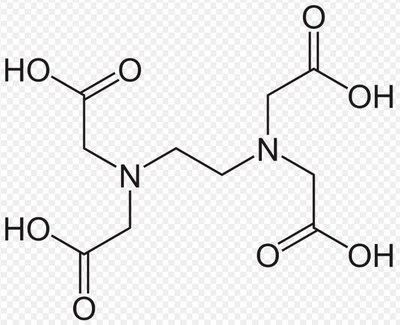
\includegraphics[scale = 0.4]{edta.png}\\
	\end{tabular}
	\caption{En haut à gauche : ligands monodentates, en haut à droite : éthylènediamine. En bas à 			gauche, ion $\text{Y}^{4-}$, base conjuguée de l'EDTA en bas à droite.}
	\end{center}
\end{figure}

\subsubsection*{Indice de coordination}

Contrairement à une liaison covalente classique, dans laquelle chacun des deux atomes fournit un électron, les ligands sont reliés à l'atome/ion central par une \textbf{liaison covalente de coordination} : le ligand donne les deux électrons de la liaison, via l'un de ses doublets non-liants, à l'atome central qui les accepte.\\

L'\textbf{indice de coordination d'un complexe} est le nombre de liaisons formées par l'atome ou l'ion central avec les ligands. Prenons deux exemples : le cisplatine (cis-diaminedichloroplatine(II) (CDDP)), d'indice de coordination 4, utilisé en traitement anticancéreux  et l'ion hexaaquafer(III) $[{\text{Fe}(\text{H}_2\text{O})_6}^{3+}]$ d'indice de coordination 6 :

\begin{figure}[h!]
	\begin{center}
		\begin{tabular}{cc}
  		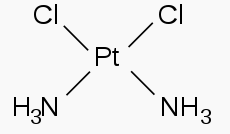
\includegraphics[scale = 0.4]{cisplatine.png} &
   		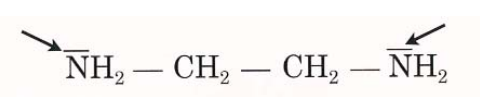
\includegraphics[scale = 0.4]{ethylenediamine.png}\\
	\end{tabular}
	\caption{Gauche : cisplatine. Droite : ion hexaaquafer(III).}
	\end{center}
\end{figure}

\subsection{Réaction de formation d'un complexe (Le Maréchal Tome 1, p99. 7.3.1)}

En guise d'introduction, on propose la synthèse de plusieurs complexes en tubes à essais
\subsubsection*{Matériel :}
\begin{itemize}
	\item 4 tubes à essais,
	\item solution de sulfate de cuivre (5\%),
	\item solution d'acide chlorhydrique à $12\;\text{mol}/\text{L}^{-1}$,
	\item solution d'ammoniac à $14\;\text{mol}/\text{L}^{-1}$. 
\end{itemize}

\subsubsection*{Protocole :}
\begin{itemize}
	\item \textbf{Tube 1 :} 1 mL de sulfate de cuivre.\\
	\item \textbf{Tube 2 :} 1 mL de sulfate de cuivre, quelques gouttes d'acide chlorhydrique 				jusqu'à l'apparition d'une couleur verte traduisant la formation du complexe :
	\begin{equation}
		\text{Cu}^{2+}_\text{(aq)} + 4\;\text{Cl}^- = [\text{CuCl}_4]^{2-}
	\end{equation}
	\item \textbf{Tube 3 :} 1 mL de sulfate de cuivre, quelques gouttes d'ammoniac, un précipité 		blanc apparaît. L'augmentation du pH, liée à l'introduction d'ammoniac et donc la production 		d'ions hydroxyde provoque la précipitation du cuivre, selon la réaction (qui n'est pas une 			complexation) :
	\begin{equation}
		\text{Cu}^{2+}_\text{(aq)} + 2\text{HO}^- = \text{Cu(OH)}_{2,\text{(s)}}
	\end{equation}
	\item \textbf{Tube 4 :} 1 mL de sulfate de cuivre, \textbf{excès d'ammoniac}. Les ligands 			hydroxyde et ammoniac sont en \textbf{compétition}. Le précipité d'hydroxyde se forme, mais en 		ajoutant suffisamment d'ammoniac, on observe sa \textbf{redissolution} et la formation d'un 		composé bleu vif (\textbf{bleu céleste}) selon la réaction
	\begin{equation}
		\text{Cu}^{2+} + 4\;\text{NH}_3 = [\text{Cu}{(\text{NH}_3)}_4]^{2+}.
	\end{equation}
	En se complexant avec le cuivre, l'ammoniac réduit la concentration en ions cuivreux dans la 		solution, améliorant leur solubilité, d'où la redissolution du précipité.
\end{itemize}

Profitons-en pour souligner que les complexes sont \textbf{souvent des molécules colorées}, et qu'ils peuvent être chargés. Dans les exemples proposés, on a un complexe chargé positivement et un complexe chargé négativement.\\

En résumé, dans une solution aqueuse, un ion métallique noté M réagit avec n ligands notés L, pour former le complexe $[\text{ML}_n]$ selon l'équation globale :
\begin{equation}
	\boxed{\text{M}_\text{(aq)} + \text{n}\;\text{L}_\text{(aq)} = [\text{ML}_{n,\text{(aq)}}]}.
\end{equation}

On définit la \textbf{constante de formation globale d'un complexe}, fonction de la température et notée $K_f$ :
\begin{equation}
	K_f \equiv \frac{[[ML_n]]^\text{eq}}{[\text{M}]^\text{eq}[\text{L}]^{n,\text{eq}}}
\end{equation}
Elle caractérise l'équilibre de formation du complexe. Plus elle est grande, plus le complexe est stable. Rappelons qu'une constante d'équilibre est une \textcolor{red}{grandeur sans dimension et que toutes les concentrations doivent être exprimées en $\text{mol}.\text{L}^{-1}$}. Prenons comme exemple la formation du complexe bleu céleste :
\begin{equation}
	K_f = \frac{[[\text{Cu}{(\text{NH}_3)}_4]^{2+}]^\text{eq}}
	{[\text{Cu}^{2+}]^\text{eq}[\text{NH}_3]^{4,\text{eq}}}.
\end{equation}

\newpage
\subsection{Quelques exemples}

Les applications des complexes sont nombreuses et variées :
\begin{itemize}
	\item En photographie argentique, on utilise des halogénures d'argent (par exemple le bromure 		d'argent AgBr). L'image latente résultant de l'exposition est révélée par un réducteur (le 			benzène-1,4-diol également appelé hydroquinone).
	
	\begin{figure}[h!]
		\begin{center}
  		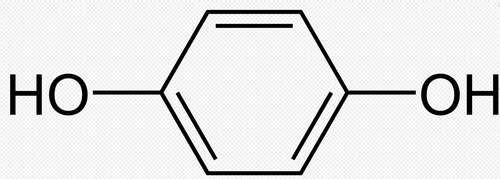
\includegraphics[scale = 0.5]{hydroquinone.png} 
		\caption{Hydroquinone.}
		\end{center}
	\end{figure}
	
	L'excès d'halogénure d'argent (non exposé, non révélé) est éliminé par complexation avec les 			ions thiosulfate(le complexe est soluble, le bromure d'argent non). C'est la fixation :
	\begin{equation}
		\text{AgBr}_\text{(s)} + 2\;{{\text{S}_2\text{O}_3}^{2-}}_\text{(aq)}
		= [\text{Ag}(\text{S}_2\text{O}_3)_2]^{3-}_\text{(aq)} + \text{Br}^{-}_\text{(aq)} 
	\end{equation}

	\item Deux complexes jouent un rôle très important dans la \textbf{vie des plantes et des 			animaux} : ce sont la \textbf{chlorophylle} et \textbf{l'hème} (un constituant de 					l'hémoglobine). Le premier est un complexe à base de magnésium jouant un rôle majeur dans la 		photosynthèse et responsable de la couleur verte des plantes. Le second est un complexe à base 		de fer, entre une porphyrine et un cation ferreux, responsable de la couleur rouge du sang. 		Dans les deux cas, le ligand est	tétradentate.\\

	Ces deux molécules sont impliquées dans le transport du dioxygène dans les organismes vivants. 		Le dioxygène peut être remplacé par le monoxyde de carbone ou par les ions cyanure, formant un 		ensemble plus stable, d'où la toxicité de ces espèces chimiques.

	\begin{figure}[h!]
		\begin{center}
  		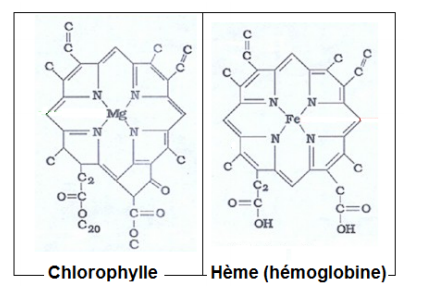
\includegraphics[scale = 0.8]{cplxbio.png} 
		\caption{Chlorophylle et hème.}
		\end{center}
	\end{figure}
	
	\item En métallurgie, on peut se servir de la capacité d'un métal à complexer pour le séparer 		d'autres métaux. Le procédé Bayer, utilisé pour traiter la bauxite en séparant ses constituants 	(essentiellement de l'alumine $\text{Al}_2\text{O}_3$ et de l'oxyde de fer(III) 
	$\text{Fe}_2\text{O}_3$), consiste à broyer la bauxite et à la plonger dans de la soude à 			chaud. Sous un pH élevé (donc en milieu très basique) l'aluminium forme un complexe soluble en 		solution aqueuse (ion tétrahydroxoaluminate(III)) selon la réaction
	\begin{equation}
		\text{Al}_2\text{O}_{3,\text{(s)}} + 2\;\text{HO}^-_\text{(aq)} 
		+ 3\;\text{H}_2\text{O}_\text{(l)} = 2\;[\text{Al(OH)}_4]^-_\text{(aq)}
	\end{equation} ce que ne fait pas le fer qui reste à l'état solide. On peut alors isoler 			l'aluminium en séparant la phase liquide de la phase solide par décantation.
\end{itemize}

\newpage
\section{Synthèse et analyse d'un complexe (Girard p3)}\label{sec:2}

On va synthétiser un complexe de l'ion cuivre(II) et utilisant le ligand oxalate 
$\text{C}_2\text{O}_4^{2-}$. La réaction de formation du complexe est la suivante
\begin{equation}
	\boxed{\text{Cu}^{2+}+2\;\text{C}_2\text{O}_4^{2-}=[\text{Cu}(\text{C}_2\text{O}_4)_2]^{2-}}.
\end{equation}

On utilise des solutions de sulfate de cuivre pentahydraté et d'oxalate de potassium monohydraté. Le produit obtenu, sous forme cristallisée, aura pour formule chimique
\begin{equation}
	\boxed{\text{K}_2[\text{Cu}(\text{C}_2\text{O}_4)_2],\text{c}\text{H}_2\text{O}.}
\end{equation} 

On veut évaluer le rendement de la synthèse et remonter à la valeur de c.

\subsection{Synthèse du complexe}

\subsubsection*{Tableau d'avancement}
La réaction de formation du complexe est la suivante \textcolor{red}{(dresser un tableau d'avancement)} :
\begin{equation}
	\boxed{\text{Cu}^{2+} + 2\;\text{C}_2\text{O}_4^{2-} + 2\;\text{K}^+ 
	+ \text{c}\;\text{H}_2\text{O}
	= \text{K}_2[\text{Cu}(\text{C}_2\text{O}_4)_2],\text{c}\;\text{H}_2\text{O}_\text{(s)}}.
\end{equation}

Rendement
\begin{equation}
	\eta \equiv \frac{\xi_f}{\xi_\text{max}}.
\end{equation}
\textcolor{red}{On calcule $\xi_\text{max}$ connaissant les quantités de matière initiales.}

\subsubsection*{Instructions}
\begin{itemize}
	\item Peser la coupelle qui contiendra le produit sec et \textbf{noter la masse}.
	\item Faire une synthèse complète en préparation, avec filtration (büchner) et séchage.
	\item Toujours en préparation, relancer une seconde synthèse et s'arrêter au refroidissement 
		à 10\degree C en préparation. \textcolor{red}{Faire la filtration en direct.}
	\item Peser le produit issu de la synthèse complète et \textbf{noter la masse}.
	\item Pas besoin de recristalliser.
\end{itemize}

\subsection{Dosage des ions oxalate}

\subsubsection*{Réaction de dosage}
\begin{equation}
	5\;\text{H}_2\text{C}_2\text{O}_4 + 2\;\text{MnO}_4^- + 6\;\text{H}_3\text{O}^+
	= 10\;\text{CO}_2 + 2\;\text{Mn}^{2+} + 14\;\text{H}_2\text{O}
\end{equation}

\begin{itemize}
	\item La mise en solution du produit cristallisé provoque sa dissolution. L'introduction 			d'acide sulfurique concentré protonne les ions oxalate en acide oxalique.
	\item Le dosage est de type rédox, entre les couples $\text{MnO}_4^{2-}/\text{Mn}^{2+}$, 
	(E\degree = 1.51 V) et $\text{CO}_{2,\text{(g)}}/\text{C}_2\text{O}_4^{2-}$ (E\degree=-0.48 V).
	\item Il faut chauffer car cette réaction, bien que thermodynamiquement très favorable, est 		lente à température ambiante.
	\item La solution s'éclaircit au cours du dosage, au fur et à mesure que le complexe est 			consommé par la réaction de titrage.
\end{itemize}	

\subsubsection*{Instructions}
\begin{itemize}
	\item Peser précisément 0.15 g de produit sec (et non 0.2 comme sur le bouquin).
	\item Dosage en direct. Relever le volume équivalent.
	\item Le volume équivalent permet de remonter à la quantité de matière en ion oxalate. On en 		déduit la quantité de matière en cuivre via la formule, puis celle en potassium grâce à 			l'électroneutralité du solide. On remonte à la quantité d'eau
	\item La différence de masse entre celle de l'échantillon et celle obtenue en utilisant les 		quantités de matière et les masses molaires de K 39.1 (g/mol), oxalate (166.2 g/mol) 
	et Cu (M = 63.5 g/mol) permet de remonter à la quantité d'eau (M = 18.0 g/mol) et donc à c.
\end{itemize}

\newpage
\section{La synthèse de l'ammoniac}\label{sec:3}

\subsection{Le procédé Haber-Bosch}

L'ammoniac est l'une des espèces chimiques parmi les plus synthétisées au monde : la production annuelle dépasse les 100 millions de tonnes. L'une des principales applications de l'ammoniac est la production d'engrais pour l'agriculture. Il intervient aussi comme précurseur dans une autre grande synthèse inorganique industrielle, celle de l'acide nitrique, lui-même utilisé dans la production d'engrais azotés.\\

En 1909, le chimiste allemand Fritz Haber réussit à transformer le diazote gazeux en ammoniac, à l'aide d'un catalyseur (constituant majoritaire l'atmosphère, le diazote est en effet un gaz inerte, pas utilisable tel quel par la majorité des organismes vivants). Quelques années plus tard, en 1913 Carl Bosch, met au point un procédé permettant d'appliquer la méthode de Haber à échelle industrielle. Cet important progrès marque le début de l'agriculture de masse, la fabrication industrielle d'engrais permettant de fertiliser des terres jusque là stériles et d'éviter d'avoir à attendre la régénération du sol.\\

De nos jours, la fabrication industrielle de l'ammoniac utilise encore ce procédé. La réaction est la suivante :
\begin{equation}
	\boxed{\text{N}_{2,\text{(g)}} + 3\;\text{H}_{2,\text{(g)}} 
	\rightleftarrows 2\;\text{NH}_{3,\text{(g)}}},
\end{equation}
catalysée par le fer $\alpha$ (maille cubique centrée) sous forme de monocristaux et la potasse. Cette synthèse s'effectue à une température de 450\degree C sous une pression énorme (250 bars). Les réacteurs doivent donc être conçus pour résister à de telles pressions, mais aussi pour évacuer la chaleur car la réaction est exothermique ($\Delta_r\text{H}\degree = -46.19 kJ/mol$). On veut éviter de dégrader le catalyseur.

\begin{figure}[h!]
	\begin{center}
  		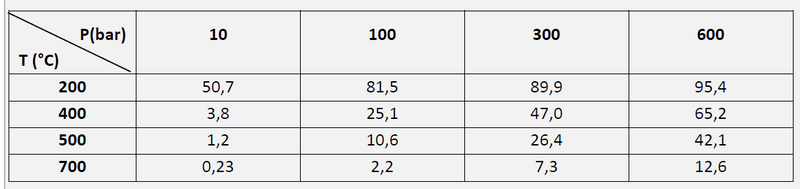
\includegraphics[scale = 0.7]{tableau_data}
		\caption{Évolution du rendement en fonction de la température et de la pression de 					travail.}
	\end{center}
\end{figure}

On remarque qu'à pression constante, augmenter la température a pour effet de réduire le rendement de la réaction. Cela s'explique par le fait que cette réaction est exothermique \textcolor{blue}{(hors programme : la loi de Van't Hoff permet de s'en rendre compte :
\begin{equation}
	\frac{d\;\text{ln}K\degree}{dt} = \frac{\Delta_r\text{H}\degree}{RT^2}).
\end{equation}
}
On pourrait se demander pourquoi on ne fait pas la réaction à température ambiante : le catalyseur, indispensable, exige une température supérieure à 400\degree C.\\

On remarque en fin qu'une augmentation de pression conduit à accroître le rendement de la réaction : c'est parce que la réaction induite une diminution du nombre total de moles de gaz \textcolor{blue}{(loi de modération de Le Châtelier, hors programme)}.

\newpage
\subsection{Mise en oeuvre industrielle du procédé Haber-Bosch}

Le diazote provient de l'atmosphère. D'où vient le dihydrogène ? Le dihydrogène est produit par vaporeformage du méthane, processus catalysé par un oxyde de nickel :
\begin{equation}
	\text{CH}_{4,\text{(g)}} + \text{H}_2\text{O}_\text{(g)} \rightleftarrows
	\text{CO}_\text{(g)} + 3\;\text{H}_{2,\text{(g)}}.
\end{equation}
Cette réaction n'est pas totale. On fait alors entrer de l'air pour déclencher la combustion du dihydrogène, portant le milieu réactionnel à une température de 1500\degree C. Cette augmentation de température permet de vaporeformer le reste du méthane, cette réaction étant endothermique (c'est l'effet contraire de celui observé pour la synthèse de l'ammoniac).

Le monoxyde de carbone réagit ensuite avec de la vapeur d'eau, produisant du dihydrogène et du dioxyde de carbone
\begin{equation}
	\text{CO}_\text{(g)} + \text{H}_2\text{O}_\text{(g)} \rightleftarrows
	\text{CO}_{2,\text{(g)}} + \text{H}_{2,\text{(g)}}.
\end{equation} 

Techniquement, on atteint un taux de conversion du diazote en ammoniac de 98\%, en faisant circuler les réactifs sur quatre lits de catalyseur et en recyclant les réactifs n'ayant pas réagi autant que nécessaire. On refroidit ensuite les gaz jusqu'à liquéfier l'ammoniac, permettant la séparation du produit et des réactifs, ces derniers étant redirigés vers le réacteur.

\begin{figure}[h!]
	\begin{center}
  		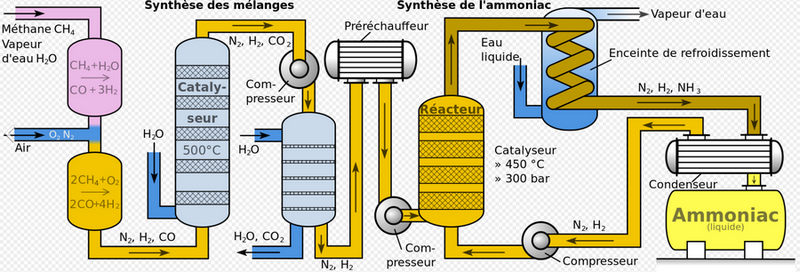
\includegraphics[scale = 0.8]{synthese_nh3.png}\\
  		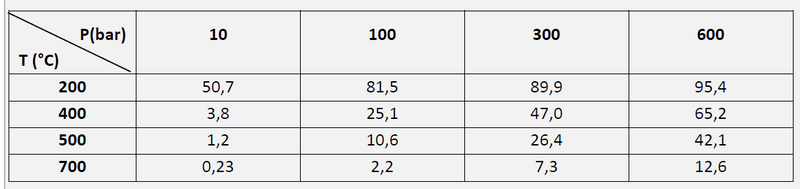
\includegraphics[scale = 0.8]{tableau_data}
		\caption{Application industrielle du procédé Haber-Bosch}
	\end{center}
\end{figure}

\section*{Conclusion}

Durant cette leçon nous avons mis en place un certain nombre de notions au sujet des complexes, des molécules très souvent colorées constituées d'un centre métallique et de ligands. Les complexes ont des applications, tant dans l'industrie que dans la biologie. Nous avons mis en oeuvre la synthèse et l'analyse quantitative d'un complexe du cuivre. Nous avons enfin présenté l'une des plus importantes synthèses inorganiques industrielles, celle de l'ammoniac. Travailler à 400\degree C sous une pression de 250 bar requiert beaucoup d'énergie. Or, certaines plantes, comme la luzerne ou le trèfle, réalisent la réaction de formation de l'ammoniac \textbf{à température ambiante}. Ceci est possible grâce à des enzymes, les nitrogénases. S'inspirer des processus biologiques (on parle de biomimétiesme) est une piste de recherche qui pourrait conduire à une chimie industrielle plus verte, moins gourmande en énergie.




\newpage
\section*{Annexes}

\subsection*{Sur les complexes du cuivre}

Ne pas oublier que les ions cuivreux sont complexés par l'eau (6 ligands) dans la solution de sulfate de cuivre. C'est ce complexe hexaaquacuivre(II) qui donne sa couleur bleue à la solution de sulfate de cuivre. Tous les cations métalliques sont solvatés et forment un aquacomplexe avec l'eau, en solution aqueuse. Les réactions de complexation sont bien souvent des substitutions de ligands.\\

On peut observer un dégagement de fumée blanche : c'est une réaction entre l'ammnoniac et le chlorure d'hydrogène gazeux, produisant du chlorure d'ammonium solide.

\subsection*{Synthèse de l'acide nitrique}

Première étape, oxydation de l'ammoniac par le dioxygène en présence d'un catalyseur (platine rhodié), réaction très exothermique
\begin{equation}
	4\;\text{NH}_3 + 5\;\text{O}_2 = 6\;\text{H}_2\text{O} + 4\;\text{NO}.
\end{equation}
Seconde étape, oxydation du monoxyde d'azote par le dioxygène
\begin{equation}
	2\;\text{NO} + \text{O}_2 = 2\;\text{NO}_2.
\end{equation}
Troisième étape, dissolution du dioxyde d'azote dans l'eau
\begin{equation}
	3\;\text{NO}_2 + \text{H}_2\text{O} = 2\;\text{HNO}_3 + \text{NO}.
\end{equation}

On recycle le monoxyde d'azote, et on distille la solution d'acide nitrique pour accroître sa concentration : on obtient un mélange de composition azéotrope au maximum (68\% d'acide, 32\% d'eau)
\end{document}